\documentclass[paper=a4, pagesize, twoside, draft=false,
BCOR7mm, DIV13, fontsize=11pt, headings=normal, footinclude=false, 
toc=listof, english, parskip=half]{scrartcl} % doppelseitiger Druck

%%%%%%%%%%%%%%%%%%%%%%%%%%%%%%%%%%%%%%%%%%%%%%%%%%%%%%%%%%%%%%%%%%%%%%%%%%%%%%%%%%%%%%%%%
%%%%%%%%%%%%%%%%%%%%%%%%%%%%%%%%%%%%%%%%%%%%%%%%%%%%%%%%%%%%%%%%%%%%%%%%%%%%%%%%%%%%%%%%
\usepackage{pyfda_style}
%%%%%%%%%%%%%%%%%%%%%%%%%%%%%%%%%%%%%%%%%%%%%%%%%%%%%%%%%%%%%%%%%%%%%%%%%%%%%%%%%%%%%%%%
%
%\includeonly{2010-DSP_FPGA-Ueb_Kap_1_2}
%
\hypersetup{
pdftitle={pyFDA: Software Architecture and Filter API},
                   pdfauthor={Christian Muenker},
                   pdfsubject={pyFDA},
                   pdfkeywords={pyFDA, filter design, python}
                   }
\def\CodePath{../pyFDA}
\def\pyFirstLine{1}
%
%
\begin{document}
%\renewmdenv[linecolor=red,frametitle={Wichtige Begriffe}]{infobox}

%\frontmatter
%%%%%%%%%%%%%%%%%%%%%%%%%%%%%%%%%%%%%%%%%%%%%%%%%%%%%%%%%%%%%%%%%%%%%%%%%%%%%%%%%%%%%%%%%
%%%%%%%%%%%%%%%%%%%%%%%%%%%%%%%%%%%%%%%%%%%%%%%%%%%%%%%%%%%%%%%%%%%%%%%%%%%%%%%%%%%%%%%%%
\author{Prof. Dr. Christian M�nker}
\title{pyFDA: Software Architecture and Filter API}
\date{\today}
%\maketitle
\begin{titlepage}
\begin{center}
\begin{Huge}pyFDA: Software Architecture and Filter API\end{Huge}
\\[1cm]
\LARGE Christian M\"unker
\vfill
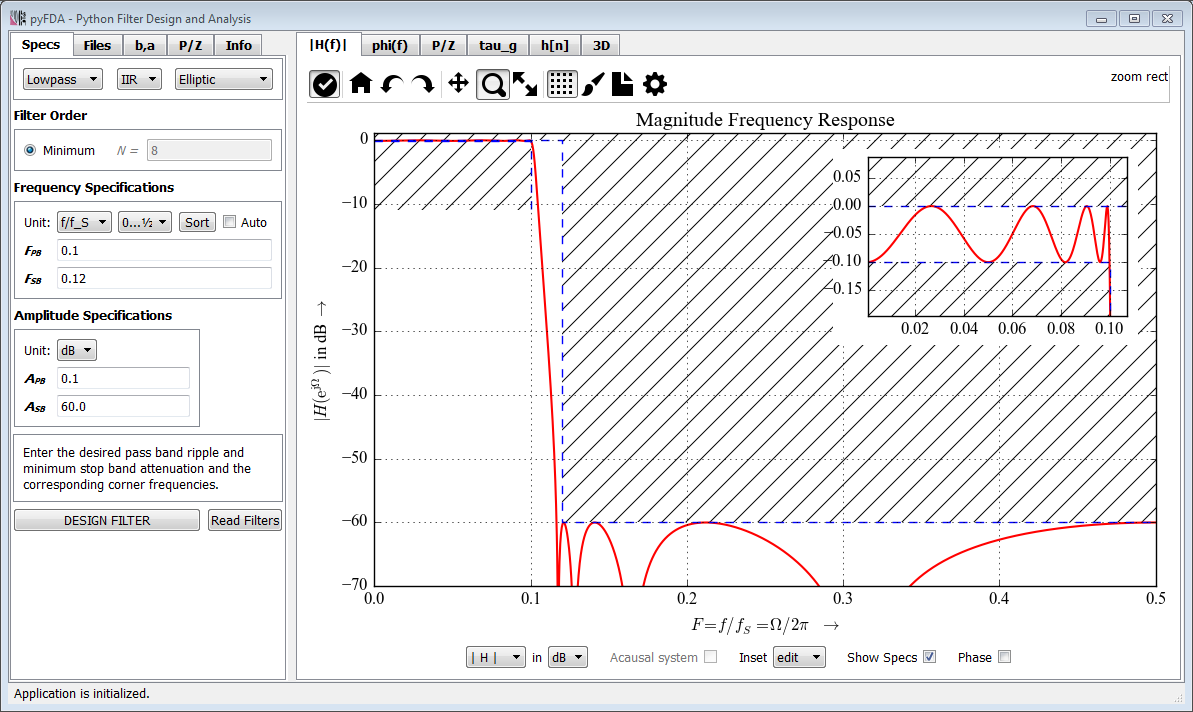
\includegraphics[width=13cm]{pyFDA_screenshot_3}

\footnotesize{pyFDA screenshot}
\vfill
\Large \today \\[1cm]
\href{mailto:Christian.Muenker@hm.edu}{Christian.Muenker@hm.edu}
\end{center}
\end{titlepage}

%
%***********************************************************************%
%*******               TABLE OF CONTENTS                        ********%
%***************                                        ****************%
\clearpage
\phantomsection % needed for correct TOC and hyperlinks
\tableofcontents
\addcontentsline{toc}{section}{Table of Contents}

%
%\def\thesection{\arabic{chapter}.\arabic{section}} 
%\include{DSP_FPGA-Ueb_Changes}
%\addcontentsline{toc}{chapter}{�nderungen}

%\def\thesection{Aufgabe \arabic{chapter}.\arabic{section}} 

%\setcounter{lofdepth}{2} % List of figures mit subfigures


%%%%%%%%%%%%%%%%%%%%%%%%%%%%%%%%%%%%%%%%%%%%%%%%%%%%%%%%%%%%%
\setcounter{topnumber}{3} % max. Anzahl von Gleitobjekten im oberen Teil der Seite

\section{Overview}
pyFDA has been written to be extensible and modular, easing the addition of own filter and analysis modules. 

This has (hopefully) been achieved with three central concepts:
\begin{description}
\item[Data persistence in a central global dictionary:] The file \textbt{filterbroker.py} with module-level attributes (dictionaries) is imported by all files that need to store and exchange parameters, filter designs etc. (\url{https://docs.python.org/3/faq/programming.html#how-do-i-share-global-variables-across-modules}). This global dictionary is also saved to / loaded from disk using (c)Pickle.
\item[Hierarchical signaling:] As the number of input, plot and design widgets increases, it gets harder to track which widgets need to be updated when. Hence, the information is collected at each hierarchical level and propagated upwards resp. received and distributed downwards.
\item[Dynamically imported design files:] A tree with all available filter design classes and characteristics is built at the start of the program from all files in the \texttt{filter\_widgets} directory. The actual classes with the design algorithms are imported dynamically when needed, the GUI is adapted according to the parameters defined in each filter design class. Additional widgets can be defined in the design class.
\end{description}
\subsection{Class Structure and Hierarchy}
The following graphics have been created from the top directory using \textbt{pyreverse} and some post-processing with LibreOffice (and they are only readable when zoomed in):

\texttt{pyreverse -o pdf -k --ignore=simpleeval.py,input\_target\_spec.py -p pyFDA .}

where 
\texttt{-k} only shows the class names (not the attributes and methods)
\texttt{-p} sets the project name that is the base for the filenames


\begin{figure}[ht]
\centering
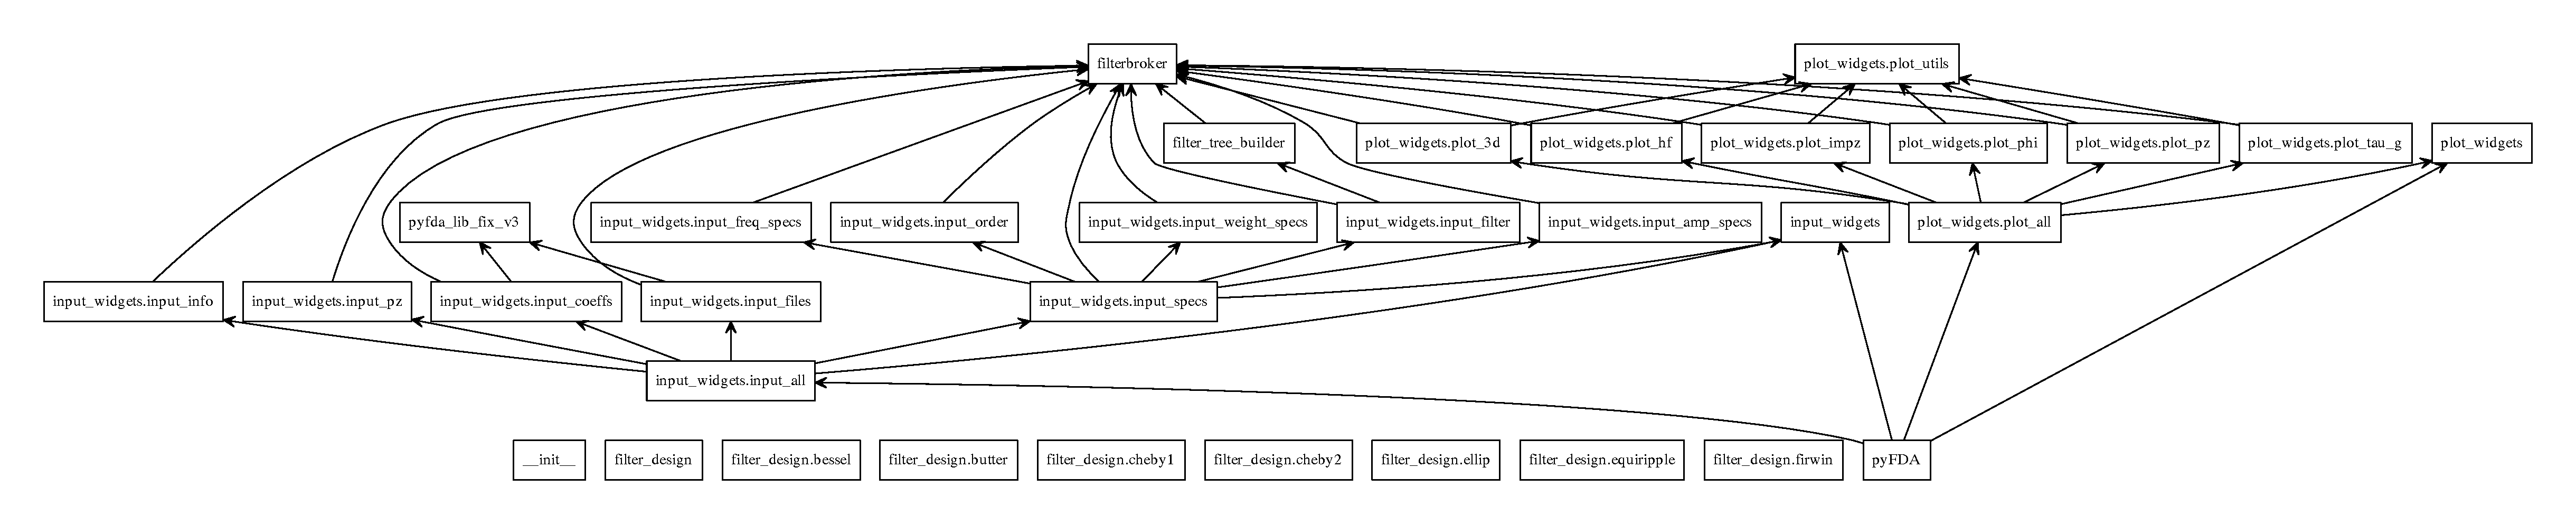
\includegraphics[width = \textwidth]{packages_pyFDA}
\caption{Packages in pyFDA}
\end{figure}

\begin{figure}[ht]
\centering
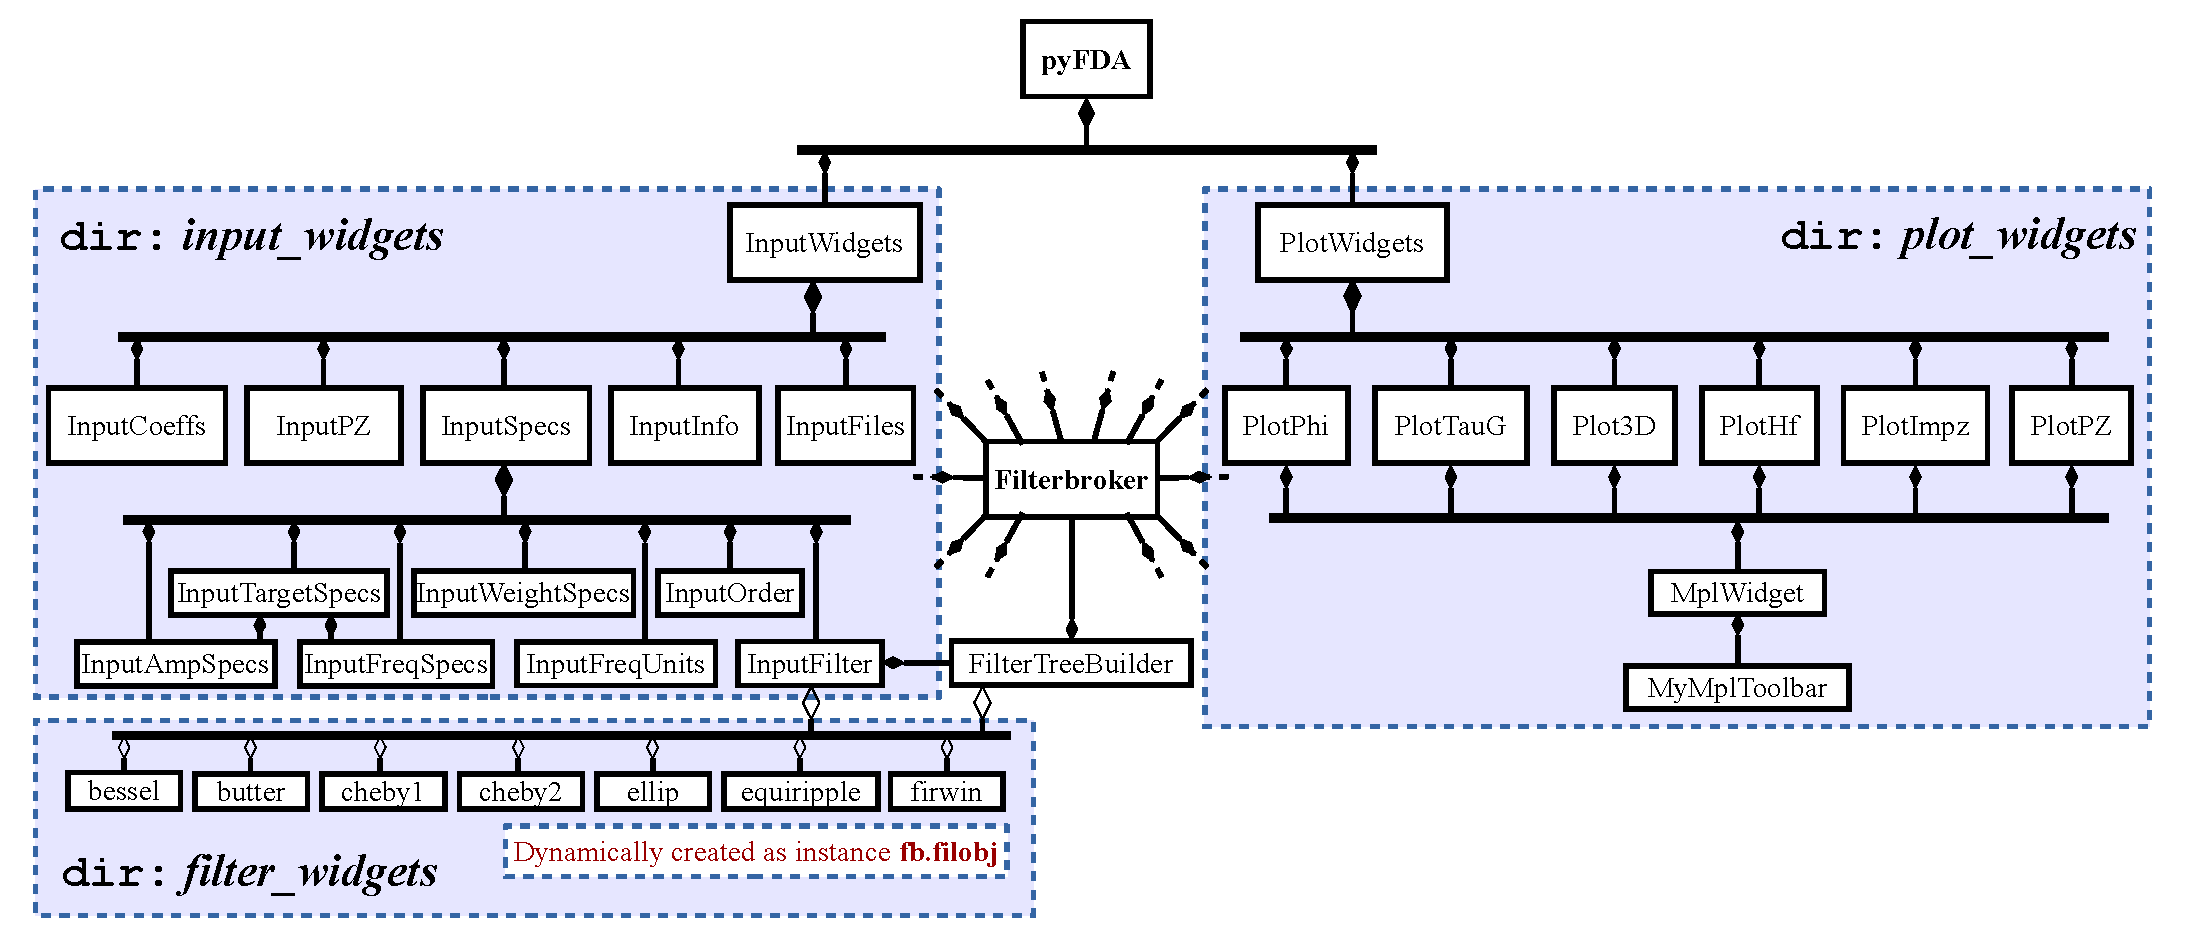
\includegraphics[width = \textwidth]{classes_pyFDA}
\caption{Class hierarchy in pyFDA (composition diagram)}
\end{figure}


\subsection{Libraries and Testing}
No proper testing strategy has been implemented so far (sorry!). However, all files / custom widgets can be run independently to test for syntactic correctness and basic functionality, especially of GUI elements. This has been achieved by the technique described in \url{http://stackoverflow.com/questions/11536764/attempted-relative-import-in-non-package-even-with-init-py} :
\begin{quotation}
"`The python import mechanism works relative to the \verb|__name__| of the current file. When you execute a file directly, it doesn't have it's usual name, but has \verb|"__main__"| as its name instead. So relative imports don't work.

You can use \verb|import some_library| directly if you have this above your imports:
\begin{lstlisting}[style = pyStyle]
if __name__ == '__main__' and __package__ is None:
    from os import sys, path
    sys.path.append(path.dirname(path.dirname(path.abspath(__file__))))
\end{lstlisting}

You can use the \verb|__package__| attribute to ensure that an executable script files in a package can relatively import other modules from within the same package. The \verb|__package__| attribute tells that file what name it's supposed to have in the package hierarchy. See \url{http://www.python.org/dev/peps/pep-0366/} for details."'
\end{quotation}

In this project, the following libraries and common files from the top level directory are used:

\begin{description}
\item [filterbroker.py] : This is the central file used as the data exchange hub where global dictionaries are defined (see section xxx). 
\item [pyfda\_lib.py] : This library contains some DSP and general helper functions.
\item [pyfda\_fixlib.py] : This library contains the fast fixpoint classes and methods.
\item [simpleeval.py] : With the help of this library simple expressions can be evaluated in line edit fields (see section xxx).
\end{description}

\begin{quotation}
"`If you have a script \verb|script.py| in package \verb|pack.subpack|, then setting it's \verb|__package__| to \verb|pack.subpack| will let you do \verb|from ..module import something| to import something from \verb|pack.module|. Note that, as the documentation says, you still have to have the top-level package on the system path. This is already the way things work for imported modules. The only thing \verb|__package__| does is let you use that behavior for directly-executed scripts as well."'
\end{quotation}

Another option is using the \verb|-m| option of the python interpreter. However, you can't run \verb|python -m core_test| from within the \verb|tests| subdirectory - it has to be from the parent, or you have to add the parent to the path. 
	

\subsection{Naming Conventions}
The following conventions have been adopted for naming instance names of UI widgets and layouts:\\
\begin{tabular}{ll}
\textbf{QtGui Widgets}\\
lblXXX: &QLabels\\
cmbXXX: &QComboBox\\
chkXXX: &QCheckBox\\
butXXX: &QPushButton\\
tblXXX: &QTableWidget\\
frmXXX:	&QFrame\\
ledXXX:	&QLineedit\\
tabXXX:	&QTabWidget\\
spcXXX:	&QSpacerItem\\
\textbf{QtGui Layouts}\\
layVXXX: &QVBoxLayout\\
layHXXX: &QHBoxLayout\\
layGXXX: &QGridLayout\\
\textbf{QtCore}
sigXXX &Signals\\
\end{tabular}

\subsection{simpleeval}

\section{Input Widgets}

\section{Plot Widgets}

\section{Signaling}
When a filter design has been changed, this information is propagated through the hierarchy to various input and plot widgets using Qt's signal-slot mechanism. 

\begin{figure}[ht]
\centering
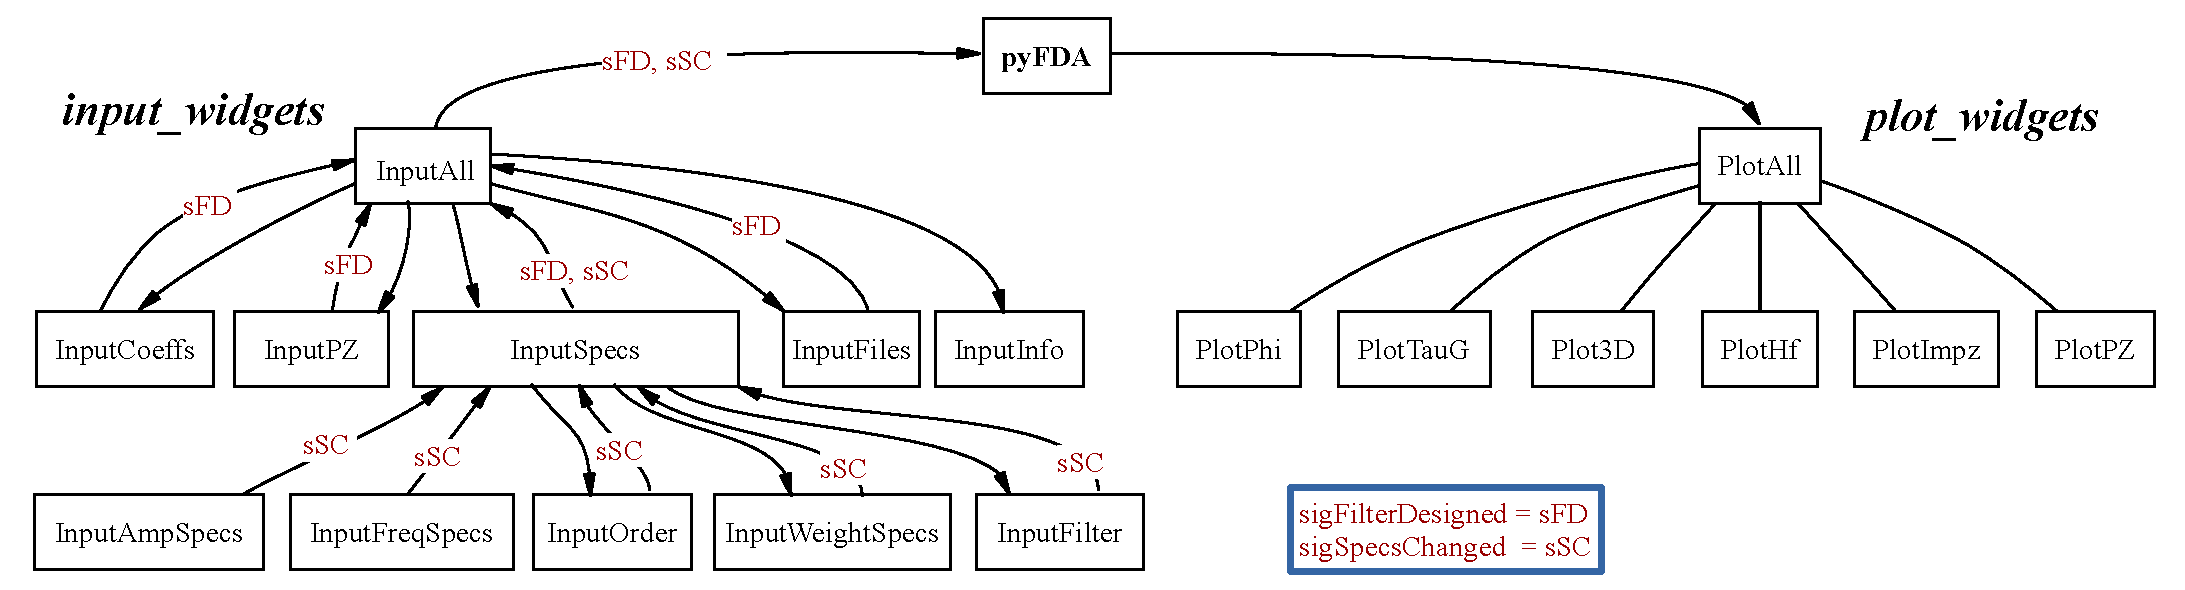
\includegraphics[width = \textwidth]{pyFDA_signals}
\caption{Signaling across hierarchies in pyFDA}
\end{figure}


Individual widgets generate signals when the filter specs have been changed or a new filter has been designed:
\begin{lstlisting}[style = pySnippet]{}
from PyQt4.QtCore import pyqtSignal
...
class MyTopClass(QtGui.QWidget):

	sigSpecsChanged  = pyqtSignal()
	sigFilterDesigned = pyqtSignal()
		...	
		def myInputWidget(self):
				self.sigSpecsChanged.emit()
				self.sigFilterDesigned.emit()
\end{lstlisting}

where \textbt{sigSpecsChanged} signifies that specifications have been changed (no replot necessary) and \textbt{sigFilterDesigned} that the filter design is finished.

\begin{figure}[ht]
\centering
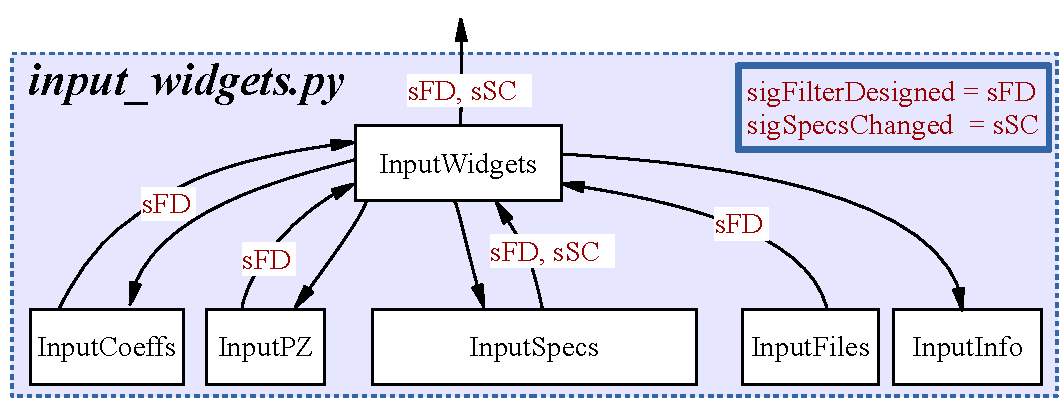
\includegraphics[width = \textwidth]{pyFDA_signals_input_widgets}
\caption{Signaling between input widgets (component: input\_widgets.py)}
\end{figure}

\section{Filter Design Objects}
The structure of a filter file and the attributes and methods that need to be provided are described in this section.

When starting pyFDA, \texttt{filter\_tree\_builder.py} is run, extracting the relevant information from all *.py files found in the subdirectory filter\_design and building a hierachical tree in \texttt{filter\_broker.py}. 


When adding new filter objects \texttt{my\_filter.py} to an pyFDA installation, two things need to be kept in mind:

\begin{itemize}
\item copying it to the \texttt{filter\_widgets} directory
\item adding a line with the filename to the list of filter files \texttt{Init.txt} in the same directory.
\end{itemize}




\subsection{Who needs you?}
A filter design object is instantiated dynamically every time the filter design method is changed in 

\texttt{input\_widgets/input\_filter.py} in \textbt{SelectFilter.setDesignMethod()}

The handle to this object is stored in \texttt{filterbroker.py} in \texttt{filObj}.

The actual design methods (LP, HP, ...) are called dynamically in \texttt{input\_widgets/input\_specs.py} in \textbt{InputSpecs.startDesignFilt()}.

An example for a design method is
\begin{lstlisting}[style = pyStyle]{}
def LPman(self, fil_dict):
	self.get_params(fil_dict)
	self.save(fil_dict, sig.ellip(self.N, self.A_PB, self.A_SB, self.F_PB, 
		btype='low', analog = False, output = frmt))
\end{lstlisting}

with the single parameter \texttt{fil\_dict}, that supplies the global filter dictionary containing all parameters and the designed filter as well. 

The local helper function \texttt{get\_params()} extracts parameters from the global filter dictionary and scales the parameters if required (as in the case for ellip routines):

\begin{lstlisting}[style = pyStyle]{}
def get_params(self, fil_dict):
 """
 Translate parameters from the passed dictionary to instance
 parameters, scaling / transforming them if needed.
 """
 self.N     = fil_dict['N']
 self.F_PB  = fil_dict['F_PB'] * 2 # Frequencies are normalized to f_Nyq
\end{lstlisting}

The local helper function \texttt{save()} saves the filter design back to the dictionary and the filter order and corner frequencies if they have been calculated by a minimum order algorithm.

\begin{lstlisting}[style = pyStyle]{}
def save(self, fil_dict, arg):
  """
  Store results of filter design in the global filter dictionary. Corner
  frequencies calculated for minimum filter order are also stored in the 
  dictionary to allow for a smooth manual filter design.
  """
  pyfda_lib.save_fil(fil_dict, arg, frmt, __name__)

  if self.F_PBC is not None: # has corner frequency been calculated?
    fil_dict['N'] = self.N # yes, update filterbroker
    if np.isscalar(self.F_PBC): # HP or LP - a single corner frequency
      fil_dict['F_PBC'] = self.F_PBC / 2.
    else: # BP or BS - two corner frequencies (BP or BS)
      fil_dict['F_PBC'] = self.F_PBC[0] / 2.
      fil_dict['F_PBC2'] = self.F_PBC[1] / 2.
\end{lstlisting}

The method

\subsection{Info strings}
All information that is displayed in \texttt{input\_widget/input\_info.py} in a \texttt{QtGui.QTextBrowser()} widget is provided in the multi line strings \textbt{self.info} and \textbt{self.info\_doc} in MarkDown format. They are analyzed and converted to HTML using \texttt{publish\_string} from \texttt{docutils.core}. \texttt{self.info} contains self-written information on the filter design method, \texttt{self.info\_doc} optionally collects python docstrings. See an excerpt from \texttt{ellip.py}:
 
\begin{lstlisting}[style=pyStyle]{}
self.info = """
**Elliptic filters**

(also known as Cauer filters) have a constant ripple :math:`A_PB` resp.
:math:`A_SB` in both pass- and stopband(s).

For the filter design, the order :math:`N`, minimum stopband attenuation
:math:`A_SB`, the passband ripple :math:`A_PB` and
the critical frequency / frequencies :math:`F_PB` where the gain drops below
:math:`-A_PB` have to be specified.

**Design routines:**

``scipy.signal.ellip()``
``scipy.signal.ellipord()``
"""

self.info_doc = []
self.info_doc.append('ellip()\n========')
self.info_doc.append(sig.ellip.__doc__)
self.info_doc.append('ellipord()\n==========')
self.info_doc.append(ellipord.__doc__)
\end{lstlisting}


\end{document}
